% !TEX encoding = UTF-8 Unicode
\documentclass[a4paper, 11pt]{article}
\usepackage[utf8]{inputenc}
\usepackage[T1]{fontenc}
\usepackage[francais]{babel}
\usepackage{fullpage}
\usepackage{hyperref}
\usepackage{graphicx}
\usepackage[nonumberlist]{glossaries}
\usepackage{amssymb,amsmath}
\makeglossaries

\title{{INFO-H-303 : Base de données} \\ Projet - Remise de la première partie}
\author{Thomas \textsc{Herman} \\ Jérôme \textsc{Hellinckx}}


\begin{document}
\maketitle

\section{Modèle entité-association}
\begin{center}
	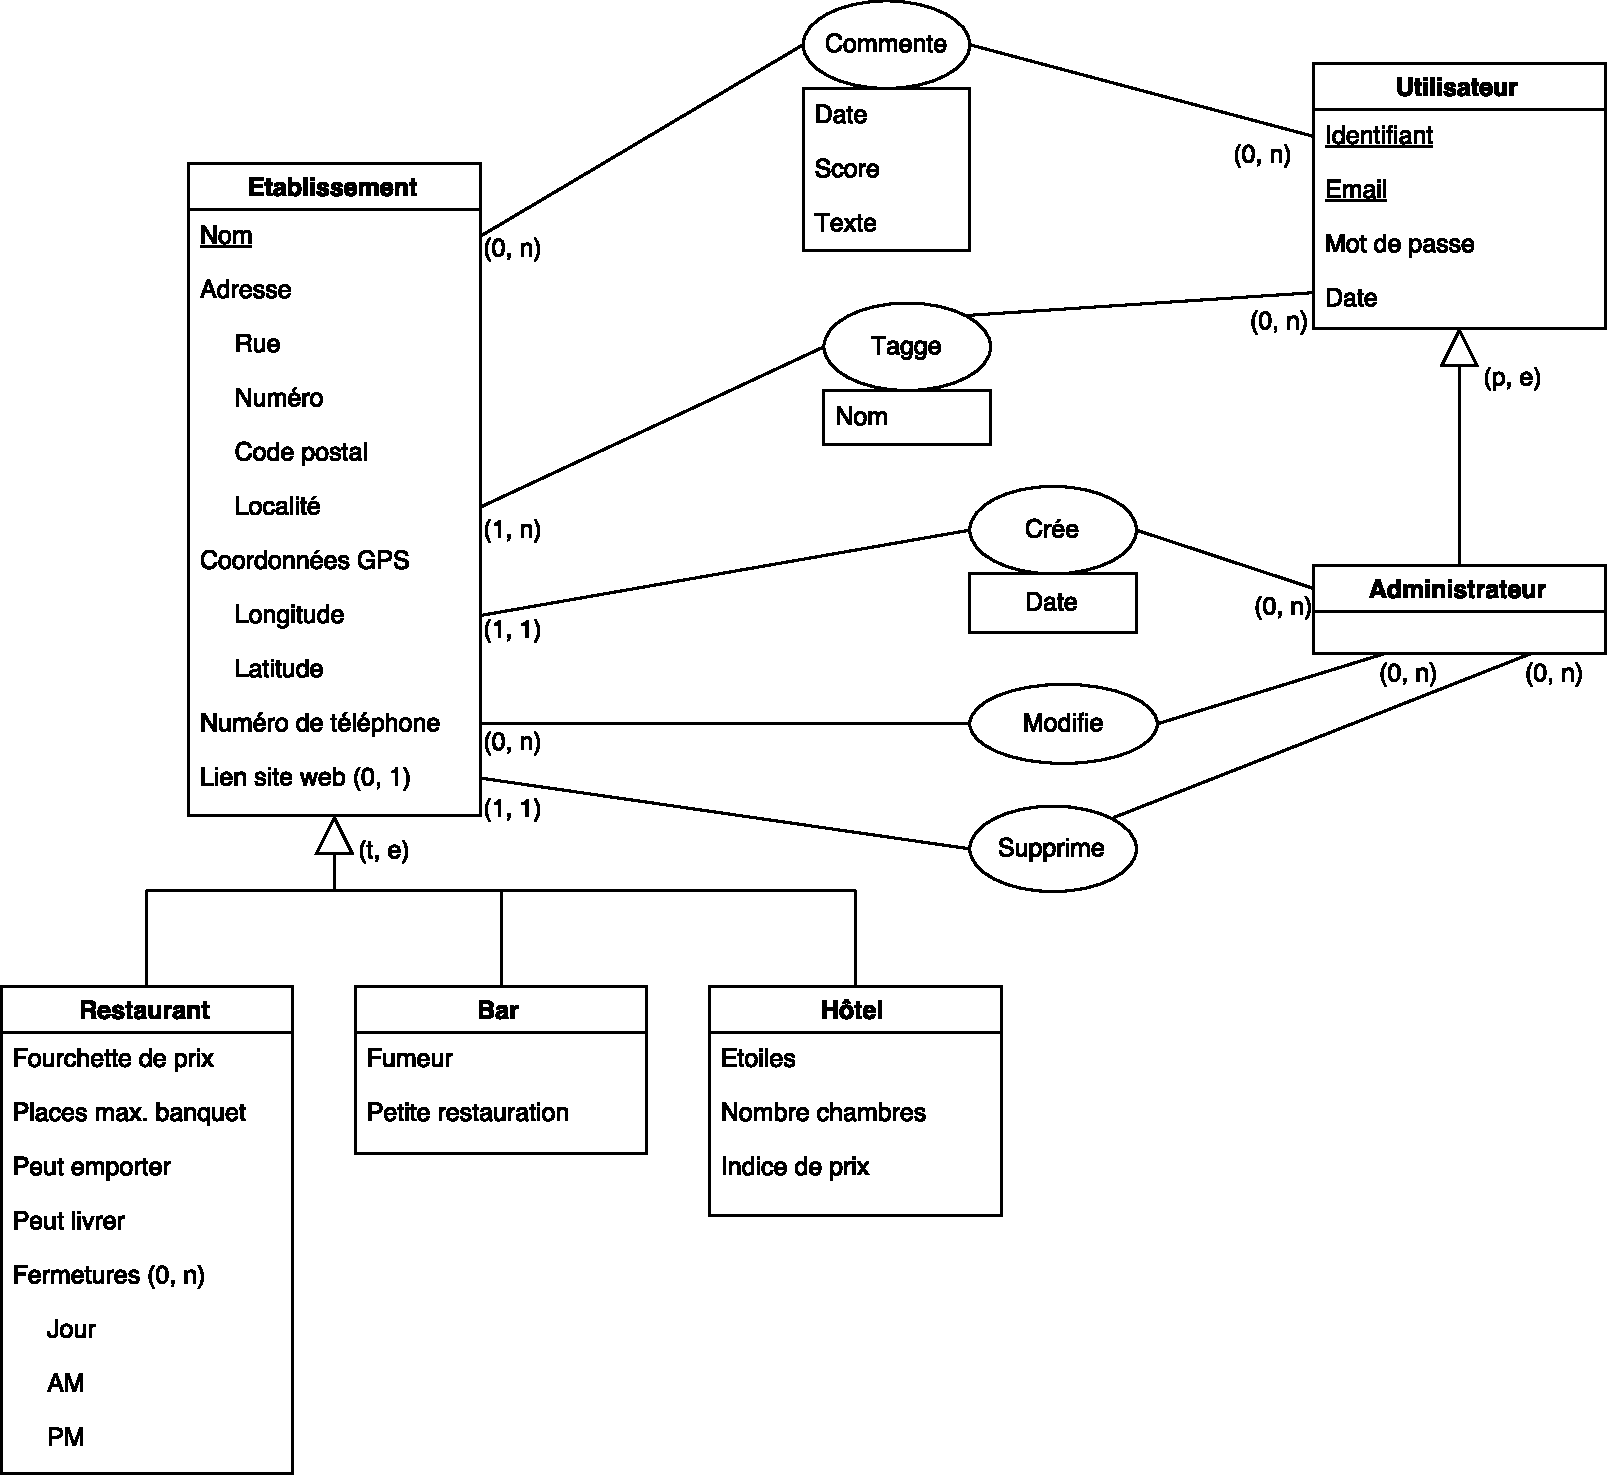
\includegraphics[scale=0.6]{horecaEA}
\end{center}

\section{Contraintes d'intégrité}

\begin{itemize}
	\item[$\bullet$] L'adresse doit se trouver dans Bruxelles (même chose pour les coordonnées GPS).
	\item[$\bullet$] L'identifiant et l'adresse email d'un utilisateur sont uniques.
	\item[$\bullet$] La date d'enregistrement d'un utilisateur précède celle d'ajout de ses commentaires. 
	\item[$\bullet$] La date d'enregistrement d'un utilisateur précède celle de création de ses établissements.
	\item[$\bullet$] La date de création d'un établissement précède tous les commentaires qui le concernent.
	\item[$\bullet$] Le score dont est composé un commentaire est compris entre 0 et 5.
	\item[$\bullet$] Un utilisateur ne peut pas commenter un même établissement 2 fois le même jour.
	\item[$\bullet$] Un utilisateur ne peut pas tagger un établissement si ce dernier possède déjà ledit tag.
	\item[$\bullet$] Un restaurant ne peut avoir plus de 14 demi journées de fermeture.
	\item[$\bullet$] Un hôtel a entre 0 et 5 étoiles.
\end{itemize}

\section{Modèle relationnel}

\end{document}